Hvis det er en økende mengde av absorbert CO\textsubscript{2} i væskefasen vil $\alpha$ øke i følge ligning \ref{loading}. Økende $\alpha$ vil også gi et økende partialtrykk av CO\textsubscript{2} i følge ligning \ref{co2loading}. Dette er illustert i figur \ref{PlotCO2abs}. 

\begin{figure}[h]  
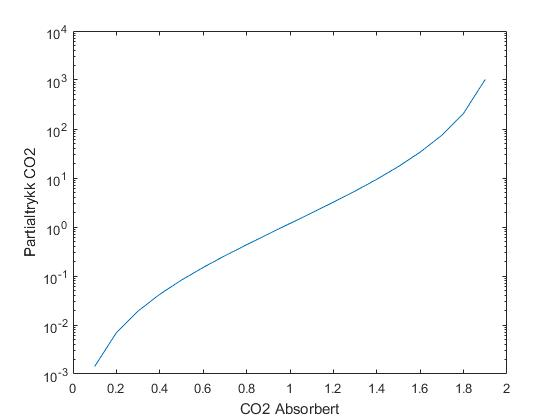
\includegraphics[scale=0.5]{Partialtrykkmotabsorbert.jpg}
\centering
\caption{Partialtrykket til CO\textsubscript{2} i bar plottet mot mol CO\textsubscript{2} absorbert i absorber for T=298K}
\label{PlotCO2abs}
\end{figure}

